\documentclass[a4paper, 12pt]{article}
\usepackage{geometry}
\geometry{a4paper,
total={170mm,257mm},left=2cm,right=2cm,
top=2cm,bottom=2cm}

\usepackage{mathtext}
\usepackage{amsmath}
\usepackage[T2A]{fontenc}
\usepackage[utf8]{inputenc}
\usepackage[english,russian]{babel}
\usepackage{graphicx, float}
\usepackage{tabularx, colortbl}
\usepackage{caption}
\captionsetup{labelsep=period}

\newcommand{\parag}[1]{\paragraph*{#1:}}
\DeclareSymbolFont{T2Aletters}{T2A}{cmr}{m}{it}
\newcounter{Points}
\setcounter{Points}{1}
\newcommand{\point}{\arabic{Points}. \addtocounter{Points}{1}}
\newcolumntype{C}{>{\centering\arraybackslash}X}

\author{Калинин Даниил, Б01-110}
\date{\today}
\title{Лабораторная работа 4.3.1. Изучение дифракции света}

\begin{document}
\maketitle
\parindent=0cm

\parag {Цель работы}
Ознакомиться с методами наблюдения 
дифракции света.

\parag {В работе используются}
оптическая скамья, ртутная лампа, монохроматор, щели с регулируемой шириной, рамка с вертикальной нитью, двойная щель, микроскоп на поперечных салазках с микрометрическим винтом, зрительная труба.

\parag {Теоритическая справка} ~\\

\textbf{Дифракция Френеля}~\\
    \begin{figure}
        \centering
        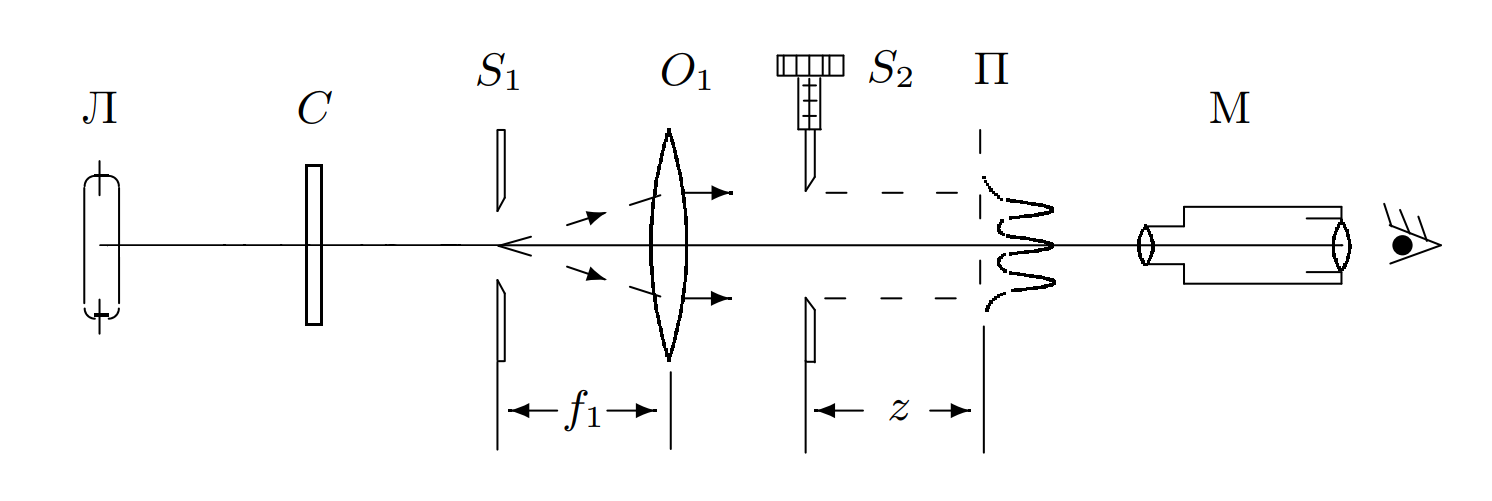
\includegraphics[width=0.6\linewidth]{fren_setup.png}
        \caption{Схема установки для наблюдения дифракции Френеля}
        \label{fig:fren_setup}
    \end{figure}

    Схема установки для наблюдения дифракции Френеля представлена на рис. \ref{fig:fren_setup}. Свет от ртутной ртутной ламы Л, пропущенный через оранжевый  ветофильтр Ф со средней длиной волны $\lambda$ = 578 нм, падает на входную щель $S_1$. Щель $S_1$ находится в фокусе коллиматора - собирающей линзы $O_1$. Коллиматор создаёт параллельный пучок монохроматического света, освещающий щель $S_2$, на которой и происходит дифракция. Дифракционная картина рассматривается с помощью микроскопа М, сфокусированного на некоторую плоскость наблюдения П.\\
    
    Распределение интенсивности света в плоскости наблюдения П проще всего рассчитывать с помощью зон Френеля (для щели их также называют зонами Шустера). При освещении щели $S_2$ параллельным пучком лучей (плоская волна) зоны Френеля представляют собой полоски, параллельные краям щели. Результирующая амплитуда в точке наблюдения определяется суперпозицией колебаний от тех зон Френеля, которые не перекрыты створками щели. Границы зон Френеля/Шустера $\xi_m$ определяется соотношением

    \begin{equation*}
        \xi_m = \pm \sqrt{mz\lambda}
    \end{equation*}
    
    где $\xi_m$ отсчитывается от центра щели, $z$ — расстояние от щели до плоскости наблюдения П, а $\lambda$ — длина волны. При ширине щели $b$ ($-\dfrac{b}{2} < \xi < \dfrac{b}{2}$) полное число открытых зон для точки наблюдения на оси равно

    \begin{equation*}
        m_{max} = \dfrac{b^2}{4 \lambda z}
    \end{equation*}
    
    Зафиксируем размер щели $b$ и проанализируем, как меняется картина в зависимости от расстояния до плоскости наблюдения z. Если число открытых зон Френеля велико, $m \gg 1$ (z $\to$ 0), мы приходим к пределу геометрической оптики. В нём дифракционная картина отсутствует, а размер изображения щели совпадает с шириной самой щели b. Дифракционная картина наблюдается только в узкой полосе вблизи границ щели («дифракция на краю экрана»). При удалении от плоскости геометрического изображения эти две группы полос постепенно расширяются, заполняя всё изображение щели. При m $\sim$ 1 на щели наблюдается сложная картина из небольшого числа дифракционных полос. При дальнейшем удалении ($m \ll 1$, z $\to$ $\infty$) дифракционная картина начинает упрощаться  и расширяться, переходя в режим Фраунгофера — затухающие по интенсивности эквидистантные полосы с характерным угловым размером центральной полосы $\dfrac{\lambda}{b}$.\\
\\
\textbf{Дифракция Фраунгофера на щели}
    \begin{figure}
        \centering
        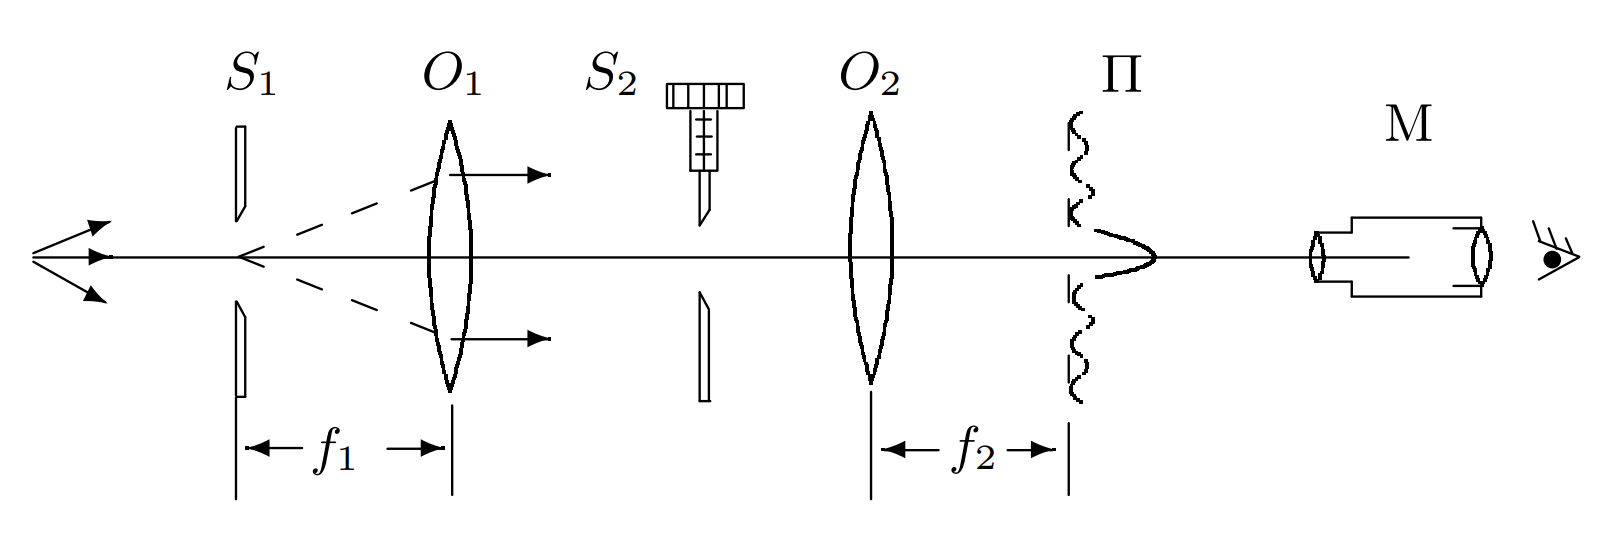
\includegraphics[width=0.6\linewidth]{fraun_one_setup.png}
        \caption{Схема установки для наблюдения дифракции Фраунгофера на одной щели}
        \label{fig:fraun_one}
    \end{figure}

    Дифракционная картина наблюдается в фокальной плоскости объектива $O_2$. Поскольку объектив не вносит дополнительной разности хода между интерферирующими лучами (таутохронизм тонкой линзы), в его фокальной плоскости наблюдается неискажённая дифракционная картина Фраунгофера, соответствующая бесконечно удалённой плоскости наблюдения. При дифракции Фраунгофера в центре поля зрения наблюдается дифракционный максимум (светлая полоса). Сбоку от неё наблюдаются чередующиеся минимумы и максимумы с довольно быстро затухающей интенсивностью. Направление на минимумы (тёмные полосы) при малых углах $\theta$ определяется соотношением 
    
    \begin{equation*}
        \theta^{min}_n = n\dfrac{\lambda}{b}
    \end{equation*}

    где b — ширина щели. Каждому значению угла $\theta$ соответствует 
    точка в плоскости объектива с фокусным расстоянием $f_2$, 
    отстоящая от оптической оси на расстоянии

    \begin{equation*}
        X_n = f_2tg(\theta_n) \approx f_2 \theta_n
    \end{equation*}

    \textbf{Дифракция фраунгофера на 2-х щелях}
    \begin{figure}
        \centering
        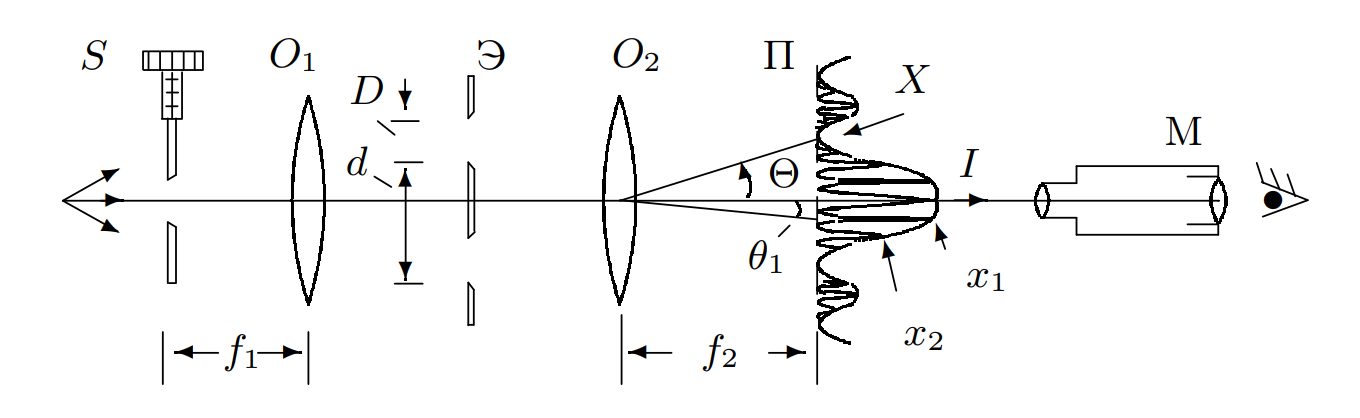
\includegraphics[width=0.6\linewidth]{fraun_two_setup.png}
        \caption{Схема установки для наблюдения дифракции Фраунгофера на двух щелях}
        \label{fig:fraun_two}
    \end{figure}

    Если входная щель достаточно узка, то дифракционная картина в     плоскости П подобна той, что получалась при дифракции на одной     щели, однако теперь вся картина испещрена рядом дополнительных     узких полос. Наличие этих полос объясняется суперпозицией (интерференцией) световых волн, приходящих в плоскость наблюдения через разные щели экрана Э. В центре главного дифракционного максимума располагается светлая полоса (разность 
    на оси, в силу симметрии, равна нулю). Светлая интерференционная полоса наблюдается также, когда разность хода кратна длине волны. Линейное расстояние $\delta x$ между соседними интерференционными полосами в плоскости П равно
    
    \begin{equation*}
        \delta x = f_2 \dfrac{\lambda}{d}
    \end{equation*}

    Штриховой линией (в увеличенном масштабе) изображено распределение    интенсивности при дифракции света на одиночной щели. Поскольку полная угловая ширина главного дифракционного максимума (от минимума до минимума) равна $\dfrac{2\lambda}{D}$, где D — ширина отдельной щели, то на нём укладывается $N = \dfrac{2d}{D}$ тёмных интерференционных полос (в центре картины максимум, поэтому светлых полос — на одну больше).

\parag {Ход работы} ~\\
    \textbf{1. Дифракция Френеля}
    
        \point Собираем установку согласно схеме.
        
        \point Настраиваем зрительную трубу на бесконечность, для этого наводим её на дальний объект и, крутя регулировочный винт, добиваемся чёткого изображения, устанавливаем зрительную трубу на скамью.
        
        \point Двигая линзу добиваемся чёткого изображения щели в зрительной
        трубе. Закрепляем линзу и первую щель.
        
        \point Ищем ноль микрометрического винта 2-й щели (момент когда она 
        открывается) (0.025мм). Закрепляем 2-ю щель за линзой, устанавливаем 
        ширину щели 0.3 мм (показания микровинта).
        
        \point Фокусируем микроскоп на щель, для этого сначала убеждаемся, что окулярная шкала видна чётко, затем, перемещая микроскоп, добиваемся чёткого изображения щели.
        
        \point Чёткое изображение - 53.9 см.

        \begin{table}[h]
            \centering
            \begin{tabular}{|c|c|c|c|c|c|c|c|c|c|c|}
                \hline
                Число полос, $m$ & 2 & 3 & 4  & 5  & 6 & 7 \\ \hline
                Координата микроскопа, $z$, см & 51.7 & 52.7 & 53.0 & 53.2 & 53.3 & 53.4   \\ \hline
            \end{tabular}
            \caption{Результаты измерений}
            \label{tabl:results_1}
        \end{table}

        \point Измеряем ширину 2-й щели при помощи шкалы микроскопа (цена деления 0,02 мм). (0,32 мм)
        
        \point  На небольшом удалении от щели наблюдаем полосы у краёв щели (Дифракция на краю экрана).
        
        \point Зафиксируем микроском и будем наблюдать за изменением дифракционной картины при изменении ширины щели (при увеличении ширины количество полос увеличивается, расстояние между полосками дифракции на краю увеличивается)

        \point Устанавливаем вместо 2-й щели рамку с тонкой проволкой, при удалении 
        микроскопа от на фоне нити наблюдаем чётное количество чёрных полос.
        рамки.

        \point Строим график зависимости расстояния до щели z, от числа открытых зон Френеля. По наклону кривой $k$ вычисляем ширину щели $b = 2 \cdot \sqrt{k\lambda}$.
        
        \begin{figure}
            \centering
            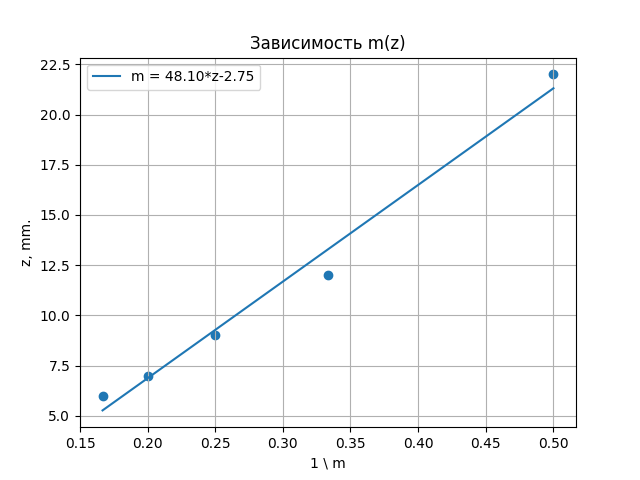
\includegraphics[width=0.6\linewidth]{plot_fren.png}
            \caption{График зависимости m(z)}
            \label{fig:plot_fren}
        \end{figure}

        Получаем: $b = 0.33 мм$\\~
        \\~
    \textbf{2. Дифракция Фраунгофера на щели}

        \point Устанавливаем между микроскопом и щелью 2-ю линзу так, чтобы микроскоп находился в фокальной плоскости 2-й линзы, для этого убираем 2-ю щель и добиваемся чёткого изображения 1-й щели в микроскопе, устанавливаем 2-ю щель, подбираем её ширину так, чтобы наблюдалась дифракционная картина.
        
        \point Ширина щели 0.36 мм, F 2-й линзы 10,2 см

        \begin{table}[h]
            \centering
            \begin{tabular}{|c|c|c|c|c|c|c|c|c|c|c|}
                \hline
            
                $m$ & -4   & -3   & -2   & -1   & 1    & 2    & 3    & 4    \\ \hline
                $X_m$, мм & 0.96 & 1.12 & 1.30 & 1.48 & 1.82 & 2.00 & 2.16 & 2.34 \\ \hline
            \end{tabular}
            \caption{Результаты измерений}
            \label{tabl:results_2}
        \end{table}

        \point При смещении щели в боковом направлении дифракционная картина не сдвигается.

        \point При увеличении ширины 2-й щели расстояние между минимумами увеличивается.

        \point Строим график зависимости положения экстремумов $x_m$ от их номера m,
        по наклону кривой k определяем ширину щели $b = \dfrac{\lambda f_2}{k}$.

        \begin{figure}
            \centering
            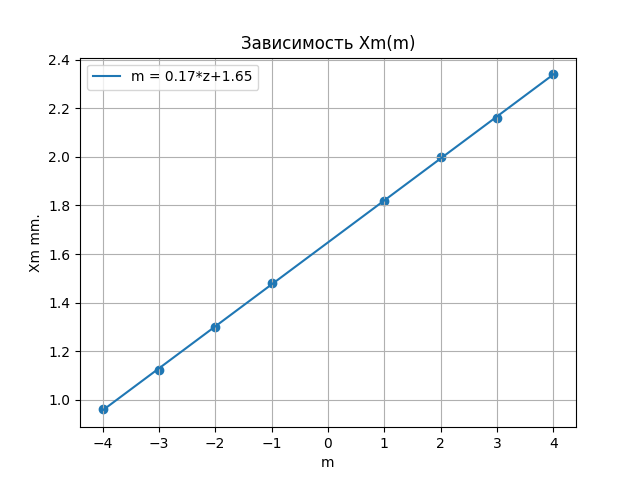
\includegraphics[width=0.6\linewidth]{plot_fraun_one.png}
            \caption{График зависимости $X_m$($m$)}
            \label{fig:plot_fraun_one}
        \end{figure}
        
        Получаем: $b = 0.340$ мм.\\~
        \\~
    \textbf{3. Дифракция Фраунгофера на двух щелях}

        \point Устанавливаем вместо 1-й щели 2-ю с микрометрическим винтом, а вместо 2-й щели пластинку с 2-мя щелями. Изменяя ширину щели S, добиваемся наибольшей чёткости изображения в микроскопе.

        \point Записываем координаты самых удалённых тёмных полос в центральном максимуем (2.20 и 2.54) и число светлых полосок между ними (7). Ширина центрального максимума - (0.92 мм)
        
        \point Подбираем такую ширину щели S $b_0$, чтобы наступило первое исчезновение интерференционных полос (0.109 мм) картина наиболее контрасна при ширине щели S (0.028 мм), а вновь появляется при ширине щели S (0.140 мм)
        
        \point F($O_1$) = 12.8 см F($O_2$) = 10.2 см

        \point $d = \dfrac{f_2 \lambda}{\delta x}$, $d = 1.21$ мм

        \point В теории количество светлых полос $= 11$, что не совпадает с  наблюдаемым их количеством.

        \point $b_0 = \dfrac{\lambda f_1}{d} = 0.061$ мм.\\~
        \\~

    \textbf{4. Влияние дифракции на разрешающую способность оптического инструмента}

        \point Устанавливаем вместо щели S рамку с 2-мя щелями, перемещая которую
        добиваемся чёткого изображения в окуляре микроскопа.

        \point Устанавливаем между линзами щель с микрометрическим винтом.

        \point Подбираем ширину щели S такую, чтобы 2 щели рамки почти сливались, но
        ещё были различимы ($b_0$ = 0.101 мм)

        \point змеряем ширину щелей $b_1$, $b_2$ и расстояние между $d$ ними при помощи микроскопа.
        ($b_{1_{left}}$ = 2.00 мм $b_{1_{right}}$ = 2.24 мм
        $b_{2_{left}}$ = 3.24 мм $b_{2_{right}}$ = 3.50 мм)



    \parag {Заключение} ~\\
        В ходе работы были исследованы явления дифракции Френеля и Фраунгофера
        на щели и 2-х щелях, а также влияние дифракции на разрешающую способность 
        оптических приборов. Часть теоретических значений совпали с практическими
        с учётом погрешностей, часть имеют существенные отличия. 
\end{document}
